%!TEX root = thesis.tex

\chapter{Commercialization}
\label{chapter6}

This work presents the initial development phases of methods using domain knowledge for model-based control and RL and the analysis of learned controllers using established control methods. These methods have the potential to provide significant economic impact to various markets that utilize robotics or automation.
%
For instance, the use of automation in industrial robotics has been shown to increase productivity while lowering output prices~\cite{Graetz:2018a}.
%
The proposed methods can further this trend since they can improve performance of existing systems with existing controllers. These methods also have the potential to accelerate the control design for new systems and applications.
%
This chapter describes some challenges and future work necessary to bring the process from this initial stage of development to a marketable process.

\section{Envisioned Market}
%
The methods proposed in this work to combine domain knowledge and RL can be introduced to a wide range of markets. Applications include any system where there is existing domain knowledge that enables model-based controllers to be developed, but where the controllers are not optimal. This may include systems that are difficult to model or applications where operating conditions are changing, in which case adaptive controllers might normally be employed. This could for instance have applications in the field robotics market, where robotic systems must be able to interact with a dynamic and unstructured environment. RL can be employed as an adaptive mechanism for various subsystems such as for manipulators interacting with payloads of unknown mass and awkward shapes or legged locomotion adapting to rough terrain~\cite{Gangapurwala:2022a}.
%
This work may also be used for applications in which controllers are necessary to account for processes that are difficult to model. For instance in the UAV market, controllers are needed to reject disturbances from wind. In these cases, a conventional model-based controller can be used to control the UAV under nominal conditions while an RL component can augment the model-based controller in the presence of disturbances~\cite{Ishihara:2023a}.

%
\begin{table}[tb]
    \begin{center}
      \setlength{\tabcolsep}{6pt}
      \caption{Technology Readiness Levels}
      \begin{tabular}{c}
      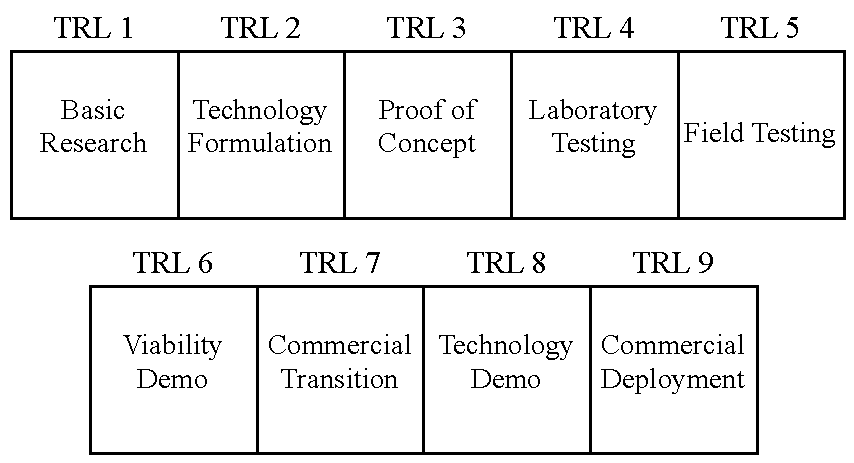
\includegraphics[width=0.8\textwidth]{figures/figures_commercialization/TRL table.pdf}
      \label{table:TRL}
      \end{tabular}
      % \vspace{-0.2in}
    \end{center}
\end{table}
%

\section{Market Viability}
The market readiness for this work can be quantified by Technology Readiness Level (TRL)~\cite{Mankins:2009a,Kimmel:2020a}. TRL was initially developed by NASA in the 1970s to describe the level of development of different systems used for space exploration. Systems had to go through rigorous testing before being deemed mission ready. The stage of development of the system can fall on a scale from 1 to 9 and characterizes systems from initial basic research principle to deployable product, as illustrated in Table~\ref{table:TRL}. The TRL method has since been adopted and modified by many other entities including the US Department of Defense and the ISO. Using this method, the TRL of the entire body of work in this dissertation is evaluated at approximately TRL 2 or TRL 3. Because of this, this work is not ready to be introduced to market. However, some parts of this work may be given a higher TRL evaluation if considered in isolation. For instance, although the methods proposed to interpret the learned controllers have low TRL,
%
the combined control methods may be categorized with a higher TRL if it was intended as an augmentation of existing products. Since the existing product and its controllers will have already gone through rigorous development and testing before being deployed, the addition of RL to the existing controller will require less development than a completely new controller.
%

\section{Increasing Market Viability}
More work is necessary to develop the concepts and methods proposed in this dissertation to increase its TRL and make it ready for market. First, this dissertation proposed multiple controller architectures to combine domain-knowledge controllers with RL and established some initial design guidelines. These different controller architectures will need to undergo more testing on various systems so that the combined controller design guidelines can be formalized.
%
In addition to general controller design, more work is needed to develop the foundational principles describing the effect of controller design and reward function design on stability. This additional development of the methods proposed in this dissertation will make the process easier for the customer to develop reliable and safe controllers.

In addition to further research needed to increase TRL, other commercial considerations must be made.
For instance, the product or service must be made user-friendly or easy to learn in order to maximize sales and profit. Also, in order for a product to be profitable, it must be divided into individual units of sale. This is challenging since the design of the combined controller using the proposed methods will need to be customized for the specific application.
%
Due to this, the proposed methods can be sold as a software package for rapid design and verification of multiple combined controller architectures.

\section{Market Challenges}
%
Although RL has already been introduced in many applications including AI-assisted design and optimization of various scheduling, allocation, and logistics problems~\cite{Kuhnle:2021a,Panzer:2022a}, many potential customers may still be hesitant to adopt RL for applications in which it is used as an adaptive controller. The performance of fixed-gain controllers can be verified for a variety of situations prior to deployment, and conventional adaptive controllers are designed to adapt in limited and predictable ways.
The use of RL and neural networks for adaptive controllers allows for a high degree of customizability to the baseline controller. However, these changes cannot be verified before deployment if these customizations are made online during operation of the system. This may prevent the adoption of the proposed work in safety critical or high risk applications.
%

\section{Impact to the Engineering Community}
%
RL alone has already been used to solve optimal control problems that cannot be solved analytically. The use of RL in this way has a very simple implementation since no domain knowledge or manual controller design is required. Although using combined controllers introduces some design complexity compared to RL alone, benefits are gained such as reduced training time and safety of the policies. Additionally, with combined controllers, model-based components can provide a foundation based on domain knowledge while the RL components account for parts of the system for which conventional optimal control design is not possible. This has the potential to reduce mechanical design constraints that are imposed by limits in conventional controller design practices such that the design of new systems may be more innovative.
%

\section{Economic Evaluation of Process}
%
The economic impact of the proposed methods can be estimated by analyzing the current growth of the global robotics market. The global robotics market in 2023 is estimated to be between approximately \$82 billion and \$114 billion with a compound annual growth rate (CAGR) between 14.7\% and 17.64\%~\cite{RoboMarket:2023a,RoboMarket:2023b}. The largest subset of the global robotics market is industrial robots. Collaborative robots, or cobots, are also a rapidly growing segment of the industrial robotics market. Cobots are required to assist humans with various tasks which will require them to quickly adapt to new situations or different humans. The methods proposed in this work can improve the efficiency of this collaboration, further increasing productivity and economic impact.
%
In addition to industrial robots, service robots are a subset of the robotics market that is expected to see significant growth in the coming years~\cite{RoboMarket:2023a}. Service robots are often utilized for inspection and maintenance, professional cleaning, and domestic tasks. Robots used for these applications will need adaptive control that can continuously optimize their behavior in unstructured and dynamic environments. The growth of this market is an indication that there is a demand for further innovation in learning controllers such that this work will have economic impact beyond the current projections.

\section{Potential Competitors}
%
With the demand to increasingly automate difficult tasks, there is a need for controllers that can provide optimal solutions for complex systems in dynamic and unstructured environments. Data-driven control methods such as RL are good candidates to provide the needed controllers for these applications. Due to this, there are several existing companies utilizing RL and ML to provide solutions for automation problems. These companies are all working to develop reliable learning controllers, making them potential competitors to the methods proposed in this dissertation.
%
